% !TeX root = RJwrapper.tex
\title{corVis: An R Package for Visualising Associations and Conditional
Associations}
\author{by Amit Chinwan and Catherine Hurley}

\maketitle

\abstract{%
Correlation matrix displays are important tools to explore multivariate
datasets. These displays with other measures of association can
summarize interesting patterns to an analyst and assist them in framing
questions while performing exploratory data analysis. In this paper, we
present new visualisation techniques to visualise association between
all the variable pairs in a dataset in a single plot, which is something
existing displays lack. Also, we propse new methods to visualise
relationship among variable pairs using conditioning. We use different
layouts like matrix or linear for our displays. We use seriation in our
displays which helps in highlighting interesting patterns easily. The R
package \texttt{corVis} provides an implementation.
}

\hypertarget{section-1-introduction}{%
\section{Section 1: Introduction}\label{section-1-introduction}}

Correlation matrix display is a popular tool to visually explore
correlations among variables while performing Exploratory Data Analysis
(EDA) on a multivariate dataset. Popularized by
\citet{friendly2002corrgrams} as corrgram, these displays are produced
by first calculating the correlation among the variables and then
plotting these calculated values in a matrix display. With effective
ordering techniques, these displays quickly highlight variables which
are highly correlated and an analyst interested in building a predictive
model could use these displays to remove correlated variables and avoid
multicollinearity.

The correlation displays are generally used with one of the Pearson's,
Spearman's or Kendall's correlation coefficient and are therefore
limited to quantitative variables. An analyst can use one-hot encoding
of the qualitative variables in order to use these displays but will
need to deal with the high dimensions as a result of the encoding. In
addition to the dimensionality problem, it is not easy to assess the
overall correlation when using the one-hot encoding. The existing
methods to quickly explore association among qualitative variables in a
dataset include using proportions or counts with different graphical
displays like boxplots or barplots. Using association measures for
qualitative pairs similar to correlation for quantitative pairs will
help in summarizing the relationship, which then can be displayed like
the correlation displays.

Tukey and Tukey introduced scagnostics which are measures for
scatterplots \citep{tukey1985computer}. Along with scagnostics, they
proposed a scagnostics scatterplot matrix which is a visual display to
explore and compare these measures for all the variable pairs in a
dataset. By comparing multiple measures at once, the unusual variable
pairs could be identified and looked at in more detail. In a similar
manner, a display comparing association measures will help in finding
interesting variable pairs. Many association measures have been proposed
to summarize different types of relationships. The most commonly used
measure is Pearson's correlation coefficient which captures any linear
trend present between the variables. Other popular measures include
Kendall's or Spearman's rank correlation coefficient which are
non-parametric measures and looks for monotonic relationship. Distance
correlation \citep{szekely2007measuring} is an important measure useful
in exploring non-linear relationships. The information theory measure
maximal information coefficient (MIC) \citep{reshef2011detecting} is
capable of summarizing complex relationships. With effective displaying
techniques, the multiple measures of association provide a comparison
tool that assist an analyst to reveal structure present in the data.

Small multiples (or Trellis display) is a simple yet powerful approach
to compare partitions of data and understand multidimensional datasets
\citep{tufte1986thevisual}. The display is produced by splitting the
data into groups by a conditioning variable and then plotting the data
for each group. Such displays allow analysts to quickly infer about the
impact of the conditioning variable. A similar idea applied to displays
of association measures (correlation plot) will help uncover underlying
patterns in the data. One such pattern is Simpson's paradox which can be
detected by comparing Pearson's correlation for data at overall level
versus individual levels of the conditioning variable.

In this paper, we propose extensions of the correlation plot and new
visualizations which look at variables of mixed type, multiple
association measures and conditional associations. These displays are
implemented in the R package \CRANpkg{corVis}. The next section provides
a review of existing packages which deal with correlation displays and a
quick background on association measures and the packages used for
calculating them. Then we describe our approach to calculate the
association measures, followed by visualizations of associations and
conditional associations. We conclude with a summary and future work.

\hypertarget{section-2-background}{%
\section{Section 2: Background}\label{section-2-background}}

In this section we provide a brief review of the existing packages used
for correlation displays and the association measures. The correlation
matrix display is an important tool to explore association among
variables in a multivariate analysis. The display was made popular by
\citet{friendly2002corrgrams} who called them corrgrams, wherein he
rendered the correlation values with shaded squares, bars, ellipses, or
circular `pac-man' symbols. The main goal of these displays is to
describe the bivariate patterns in a dataset.

\hypertarget{section-2.1-literature-review-on-correlation-displays}{%
\subsection{Section 2.1: Literature Review on Correlation
Displays}\label{section-2.1-literature-review-on-correlation-displays}}

There are various packages available in R which can be used to create
correlation matrix displays. The R package \CRANpkg{corrplot}
\citep{corrplot2021} provides an implementation of the
\citet{friendly2002corrgrams} paper. It serves as a visual exploratory
tool for correlation matrices and includes various variable ordering
methods which assist in detecting patterns of relations among the
variables. The package \CRANpkg{corrr} \citep{corrr2020} is useful in
calculating as well as visualising correlations. It calculates a
correlation \texttt{dataframe} for a dataset and hence is easier to
focus on the correlations of certain variables. The package provide
different ways to produce correlation displays. In addition to matrix
display, the package also plots the correlation values in a network
display which is useful when dealing with high-dimensional datasets.
Table \ref{tab:corrdisplay-packages} provides a list of the packages
available in R for either calculating correlations, visualising
correlations or both.

The majority of the packages in Table \ref{tab:corrdisplay-packages}
focus only on quantitative variables of the dataset. The packages
\CRANpkg{correlationfunnel} \citep{correlationfunnel} and
\CRANpkg{linkspotter} \citep{linkspotter} look at both the quantitative
as well as the qualitative variables during the correlation analysis.
\CRANpkg{correlationfunnel} speeds up the feature selection step by
looking at the relationship of predictors to a response (or a target).
It converts numeric predictors into factors, applies one-hot encoding to
all the factors and then calculates and visualise the Pearson's
correlation coefficient among the response and the predictors. On the
other hand, \CRANpkg{linkspotter} calculates different association
measures for the quantitative and qualitative variables and then uses a
network plot to visualise these association. We believe that using
different association measures is a better approach than using one-hot
encoding for exploring all the variables, as the encoding increases the
dimensions very quickly and it is not easy to assess the overall
correlation.

\begin{Schunk}
\begin{table}

\caption{\label{tab:corrdisplay-packages}List of the R packages dealing with correlation or correlation displays with information on whether the plots are seriated, interactive and are useful for high dimensions.}
\centering
\begin{tabular}[t]{l|l|l|l|l|l}
\hline
package & display & displayType & seriatedPlot & interactivePlot & highDimension\\
\hline
coreheat & heatmap & overlay & No & No & No\\
\hline
corrplot & heatmap & overlay & Yes & No & No\\
\hline
corrr & heatmap/network & facet/overlay & Yes & No & Yes\\
\hline
corrgrapher & network & overlay & No & No & Yes\\
\hline
corrarray & no display & none & No & No & No\\
\hline
correlationfunnel & funnel & overlay & No & No & Yes\\
\hline
linkspotter & network & overlay & No & Yes & Yes\\
\hline
correlation & heatmap/network & overlay & No & No & Yes\\
\hline
\end{tabular}
\end{table}

\end{Schunk}

There have been other extensions to correlation displays which are
useful when dealing with high dimensional datasets.
\citet{buja2016visualization} proposed Association Navigator which is an
interactive visualization tool for large correlation matrices with upto
2000 variables. They also provide different functionalities including
highlighting variables, plotting scatterplot for variable pairs. The R
package \CRANpkg{scorrplot2022} \citep{sCorrPlot} produces an
interactive scatterplot for exploring pairwise correlations in a large
dataset by projecting variables as points with respect to some
user-selected variables on a scatterplot, driven by geometric
interpretation of correlation. A user can update variables of interest
and can create tours of the correlation space between different
projections of the data using this tool. In this paper, we do not focus
on the high dimensionality aspect of the correlation displays like these
tools but introduce conditional association displays which are useful in
uncovering conditional structure present in the data. Conditional
displays (also called Small multiple displays or Trellis displays) are
visualisations for the subsets of data produced by dividing the data by
a partitioning variable and then plotting them. Popularised by
\citet{tufte1986thevisual} and \citet{becker1996thevisual}, these
displays are efficient for discovering interesting patterns in the data.

\hypertarget{section-2.2-literature-review-on-association-measures}{%
\subsection{Section 2.2: Literature Review on Association
Measures}\label{section-2.2-literature-review-on-association-measures}}

An association measure can be defined as a numerical summary quantifying
relationship between two or more variables. For example, Pearson's
correlation coefficient summarizes the strength and direction of the
linear relationship present between two numeric variables and is in the
range \([-1,1]\). Kendall's or Spearman's rank correlation coefficient
are other popular measures which look for the presence of montonic
relationship among two numeric variables and are in the range
\([-1,1]\). As these measures are limited to linear or monotonic
relationships, there's a need to use association measures which can
capture complex relationships (like non-linear or periodic). The
distance correlation coefficient \citep{szekely2007measuring} is one
such measure which looks for the non-linear association between two
numeric variables and summarizes it in \([0,1]\). Similarly, MIC
\citep{reshef2011detecting} is capable of summarizing non-linear as well
as periodic relationships between numeric variables. In addition to
association measures for numeric variables, association measures for
ordinal or nominal or mixed variables will help an analyst in exploring
a multivariate dataset. \citet{taha201673} provides an overview of the
association measures used for categorical or mixed data.

\citet{tukey1985computer} proposed scatterplot matrix of the scagnostics
measures, which are measures summarizing a scatterplot. They suggested
that scatterplot matrix of the measures can be used to identify unusual
scatterplots or variable pairs. \citet{wilkinson2005graph} used this
idea with their graph-theoretic scagnostic measures to highlight unusual
scatterplot. Similarly, \citet{kuhn2013applied} have used this idea in a
predictive modeling context. They have produced a scatterplot matrix of
the measures between the response and continuous predictors such as
Pearson's correlation coefficient, pseudo-\(R^2\) from the locally
weighted regression model, MIC and Spearman's rank correlation
coefficient to explore the predictor importance during feature selection
step. These displays show the importance of comparing multiple
association measures at once for different variable pairs. In this
paper, we propose different visualization techniques to compare multiple
association measures for all the variable pairs in a dataset which can
assist a user in finding interesting patterns.

\hypertarget{section-3-corvis-calculating-association}{%
\section{Section 3: corVis: Calculating
Association}\label{section-3-corvis-calculating-association}}

This section provides an implementation for the calculation of
association measures in our package \CRANpkg{corVis}. The package
provides a collection of various measures of association which is used
to quantify the relationship between two variables and is used to
explore patterns during EDA. The measures available in the package are
not limited to numeric variables and are used with categorical and
ordinal variables as well. Table \ref{tab:association-measures} lists
the different measures of association provided in the package with the
variable types they can be used with, the package used for calculation,
the information on whether the measure is symmetric, and the minimum and
maximum value of the measure.

\begin{Schunk}
\begin{table}

\caption{\label{tab:association-measures}List of the functions available in the package for calculating different association measures along with the packages used for calculation.}
\centering
\begin{tabular}[t]{l|l|l|l|l|r|r}
\hline
funName & typeX & typeY & from & symmetric & min & max\\
\hline
tbl\_cor & numeric & numeric & stats::cor & TRUE & -1 & 1\\
\hline
tbl\_dcor & numeric & numeric & energy::dcor2d & TRUE & 0 & 1\\
\hline
tbl\_mine & numeric & numeric & minerva::mine & TRUE & 0 & 1\\
\hline
tbl\_polycor & ordinal & ordinal & polycor::polychor & TRUE & -1 & 1\\
\hline
tbl\_tau & ordinal & ordinal & DescTools::KendalTauA,B,C,W & TRUE & -1 & 1\\
\hline
tbl\_gkTau & nominal & nominal & DescTools::GoodmanKruskalTau & FALSE & 0 & 1\\
\hline
tbl\_gkLambda & nominal & nominal & DescTools::GoodmanKruskalTau & TRUE & 0 & 1\\
\hline
tbl\_gkGamma & nominal & nominal & DescTools::GoodmanKruskalTau & TRUE & 0 & 1\\
\hline
tbl\_uncertainty & nominal & nominal & DescTools::UncertCoef & TRUE & 0 & 1\\
\hline
tbl\_chi & nominal & nominal & DescTools::ContCoef & TRUE & 0 & 1\\
\hline
tbl\_cancor & nominal & nominal & corVis & TRUE & 0 & 1\\
\hline
tbl\_cancor & nominal & numerical & corVis & TRUE & 0 & 1\\
\hline
tbl\_nmi & any & any & corVis & TRUE & 0 & 1\\
\hline
tbl\_easy & any & any & correlation::correlation & TRUE & -1 & 1\\
\hline
\end{tabular}
\end{table}

\end{Schunk}

\hypertarget{calculating-association-for-relevant-variables}{%
\subsection{Calculating association for relevant
variables}\label{calculating-association-for-relevant-variables}}

We introduce a method which creates a tibble structure for the variable
pairs in a dataset along with calculated association measure. The
package contains various functions (shown in Table
\ref{tab:association-measures}) for different association measures in
the form \texttt{tbl\_*} to calculate them. For example, a user might be
interested in calculating distance correlation for numeric pair of
variables in a dataset. This can be done by using \texttt{tbl\_dcor}.

\begin{Schunk}
\begin{Sinput}
df <- penguins
distance <- tbl_dcor(df)
head(distance)
\end{Sinput}
\begin{Soutput}
#> # A tibble: 6 x 4
#>   x                 y              measure measure_type
#>   <chr>             <chr>            <dbl> <chr>       
#> 1 bill_depth_mm     bill_length_mm  0.387  dcor        
#> 2 flipper_length_mm bill_length_mm  0.666  dcor        
#> 3 body_mass_g       bill_length_mm  0.587  dcor        
#> 4 year              bill_length_mm  0.0784 dcor        
#> 5 flipper_length_mm bill_depth_mm   0.704  dcor        
#> 6 body_mass_g       bill_depth_mm   0.614  dcor
\end{Soutput}
\end{Schunk}

Similarly, one can use \texttt{tbl\_nmi} to calculate normalised mutual
information for numeric, nominal and mixed pair of variables.

\begin{Schunk}
\begin{Sinput}
nmi <- tbl_nmi(df)
head(nmi)
\end{Sinput}
\begin{Soutput}
#> # A tibble: 6 x 4
#>   x                 y         measure measure_type
#>   <chr>             <chr>       <dbl> <chr>       
#> 1 island            species 0.507     nmi         
#> 2 bill_length_mm    species 0.353     nmi         
#> 3 bill_depth_mm     species 0.315     nmi         
#> 4 flipper_length_mm species 0.343     nmi         
#> 5 body_mass_g       species 0.300     nmi         
#> 6 sex               species 0.0000854 nmi
\end{Soutput}
\end{Schunk}

\hypertarget{calculating-association-measures-for-whole-dataset}{%
\subsection{Calculating association measures for whole
dataset}\label{calculating-association-measures-for-whole-dataset}}

\texttt{calc\_assoc} can be used to calculate association measures for
all the variable pairs in the dataset at once in a tibble structure. In
addition to tibble structure, the output also has \texttt{paiwise} and
\texttt{data.frame} class which are important class attributes for
producing visual summaries in this package.

The tibble output for \texttt{calc\_assoc} has the following structure:

\begin{itemize}
\tightlist
\item
  \texttt{x} and \texttt{y} representing a pair of variables
\item
  \texttt{measure} representing the calculated value for association
  measure
\item
  \texttt{measure\_type} representing the association measure calculated
  for \texttt{x} and \texttt{y} pair.
\end{itemize}

The variable pairs in the output are unique pairs and a subset of all
the variable pairs of a dataset where \texttt{x} \(\neq\) \texttt{y}. As
explained earlier, the \texttt{measure\_type} represents the association
measure calculated for a specific type of variable pair. A user can be
interested in calculating multiple association measures for a type of
variable pair. This can be done by using the \texttt{calc\_assoc} and
\texttt{update\_assoc} together for calculating different association
measures and then merging the output tibbles.

\begin{Schunk}
\begin{Sinput}
complete_assoc <- calc_assoc(df)
glimpse(complete_assoc)
\end{Sinput}
\begin{Soutput}
#> Rows: 28
#> Columns: 4
#> $ x            <chr> "island", "bill_length_mm", "bill_depth_mm", "flipper_len~
#> $ y            <chr> "species", "species", "species", "species", "species", "s~
#> $ measure      <dbl> 0.81328762, 0.84131393, 0.82447508, 0.88217284, 0.8183348~
#> $ measure_type <chr> "cancor", "cancor", "cancor", "cancor", "cancor", "cancor~
\end{Soutput}
\begin{Sinput}
class(complete_assoc)
\end{Sinput}
\begin{Soutput}
#> [1] "pairwise"   "tbl_df"     "tbl"        "data.frame"
\end{Soutput}
\end{Schunk}

The function has a \emph{types} argument which is basically a tibble of
the association measure to be calculated for different variable pairs.
The default tibble of measures is \texttt{default\_assoc()} which
calculates Pearson's correlation if both the variables are numeric,
Kendall's tau-b if both the variables are ordinal, canonical correlation
if one is factor and other is numeric and canonical correlation for the
rest of the variable pairs.

\begin{Schunk}
\begin{Sinput}
default_measures <- update_assoc()
default_measures
\end{Sinput}
\begin{Soutput}
#> # A tibble: 4 x 4
#>   funName    typeX   typeY   argList
#>   <chr>      <chr>   <chr>   <list> 
#> 1 tbl_cor    numeric numeric <NULL> 
#> 2 tbl_tau    ordered ordered <NULL> 
#> 3 tbl_cancor factor  numeric <NULL> 
#> 4 tbl_cancor other   other   <NULL>
\end{Soutput}
\end{Schunk}

An analyst can update these measures using the \texttt{update\_assoc}
function where one can specify a \texttt{tbl\_*} function to calculate
association measure depending on the variable pair in the dataset and a
method if it calculates more than one measure.

\begin{Schunk}
\begin{Sinput}
updated_assoc <- update_assoc(num_pair = "tbl_cor",
                              num_pair_argList = "spearman",
                              mixed_pair = "tbl_cancor",
                              other_pair = "tbl_nmi")
updated_assoc
\end{Sinput}
\begin{Soutput}
#> # A tibble: 4 x 4
#>   funName    typeX   typeY   argList  
#>   <chr>      <chr>   <chr>   <list>   
#> 1 tbl_cor    numeric numeric <chr [1]>
#> 2 tbl_tau    ordered ordered <NULL>   
#> 3 tbl_cancor factor  numeric <NULL>   
#> 4 tbl_nmi    other   other   <NULL>
\end{Soutput}
\begin{Sinput}
updated_complete_assoc <- calc_assoc(df, types = updated_assoc)
head(updated_complete_assoc)
\end{Sinput}
\begin{Soutput}
#> # A tibble: 6 x 4
#>   x                 y         measure measure_type
#>   <chr>             <chr>       <dbl> <chr>       
#> 1 island            species 0.507     nmi         
#> 2 bill_length_mm    species 0.841     cancor      
#> 3 bill_depth_mm     species 0.824     cancor      
#> 4 flipper_length_mm species 0.882     cancor      
#> 5 body_mass_g       species 0.818     cancor      
#> 6 sex               species 0.0000854 nmi
\end{Soutput}
\end{Schunk}

\hypertarget{calculating-conditional-association}{%
\subsection{Calculating conditional
association}\label{calculating-conditional-association}}

\texttt{calc\_assoc\_by} can be used to calculate association measures
for all the variable pairs at different levels of a categorical
variable. This can help in exploring the conditional associations and
find out interesting patterns in the data prior to modeling. The output
of this function is a tibble structure with \texttt{pairwise} and
\texttt{data.frame} as additional class attributes. The \texttt{by}
argument is used for the grouping variable which needs to be
categorical.

\begin{Schunk}
\begin{Sinput}
complete_assoc_by <- calc_assoc_by(df,by = "sex")
\end{Sinput}
\end{Schunk}

The function also has a \texttt{types} argument which can be updated
similarly to \texttt{calc\_assoc}.

\begin{Schunk}
\begin{Sinput}
updated_assoc <- update_assoc(num_pair = "tbl_cor",
                              num_pair_argList = "spearman",
                              mixed_pair = "tbl_cancor",
                              other_pair = "tbl_nmi")
updated_complete_assoc_by <- calc_assoc_by(df,by = "sex", types = updated_assoc)
head(updated_complete_assoc_by)
\end{Sinput}
\begin{Soutput}
#> # A tibble: 6 x 5
#>   x                 y       measure measure_type by    
#>   <chr>             <chr>     <dbl> <chr>        <fct> 
#> 1 island            species  0.502  nmi          female
#> 2 bill_length_mm    species  0.885  cancor       female
#> 3 bill_depth_mm     species  0.900  cancor       female
#> 4 flipper_length_mm species  0.914  cancor       female
#> 5 body_mass_g       species  0.911  cancor       female
#> 6 year              species  0.0457 cancor       female
\end{Soutput}
\end{Schunk}

By default, the function calculates the association measures for all the
variable pairs at different levels of the grouping variable and the
pairwise association measures for the ungrouped data (\emph{overall}).
This behavior can be changed by setting \texttt{include.overall} to
\emph{FALSE}.

\begin{Schunk}
\begin{Sinput}
complete_assoc_by <- calc_assoc_by(df,by = "sex",include.overall = FALSE)
\end{Sinput}
\end{Schunk}

The tibble output for \texttt{calc\_assoc\_by} has the similar structure
as \texttt{calc\_assoc} with an additional \texttt{by} column
representing the levels of the categorical variable used in the
function. The variable pairs in the output are repeated for every level
of \texttt{by} variable. At present the function doesn't allow multiple
\texttt{by} variables to be used for conditioning but is something which
can be done by using the \texttt{calc\_assoc\_by} function multiple
times and then merging the multiple outputs.For calculating multiple
measures for a specific variable type, one can use
\texttt{update\_assoc} with \texttt{calc\_assoc\_by} and then can merge
these multiple tibble outputs.

\hypertarget{section-4-corvis-visualising-association}{%
\section{Section 4: corVis: Visualising
Association}\label{section-4-corvis-visualising-association}}

We propose novel visualisations to display association for every
variable pair in a dataset in a single plot and show multiple bivariate
measures of association simultaneously to find out interesting patterns.
Efficient seriation techniques have been included to order and highlight
interesting relationships. These ordered association and conditional
association displays can help find interesting patterns in the dataset.
While designing these displays we considered matrix-type, linear and
network-based layouts. A matrix-type layout simplifies lookup, and
different measures may be displayed on the upper and lower diagonal.
Linear layouts are more space-efficient than matrix plots, but lookup is
more challenging. Variable pairs can be ordered by relevance (usually
difference in measures of association or across the factor levels), and
less relevant pairs can be omitted.

Figure \ref{fig:assoc-heatmap} shows this display for every variable
pair in the \emph{penguins} dataset from the \emph{palmerpenguins}
package. It shows a high positive Pearson's correlation among
flipper\_length\_mm and body\_mass\_g, flipper\_length\_mm and
bill\_length\_mm, and bill\_length\_mm and bodymass\_g. There seems to
be a strong negative Pearson's correlation between flipper\_length\_mm
and bill\_depth\_mm, and bill\_depth\_mm and body\_mass\_g. The plot
also shows that there is a high canonical correlation between species
and other variables except year and sex, and a high canonical
correlation between island and species, which traditional correlation
matrix display would omit as they are limited to numeric variable pairs
only. The variables in the display are ordered using average linkage
clustering method to find out highly associated variables quickly.

\begin{Schunk}
\begin{figure}

{\centering 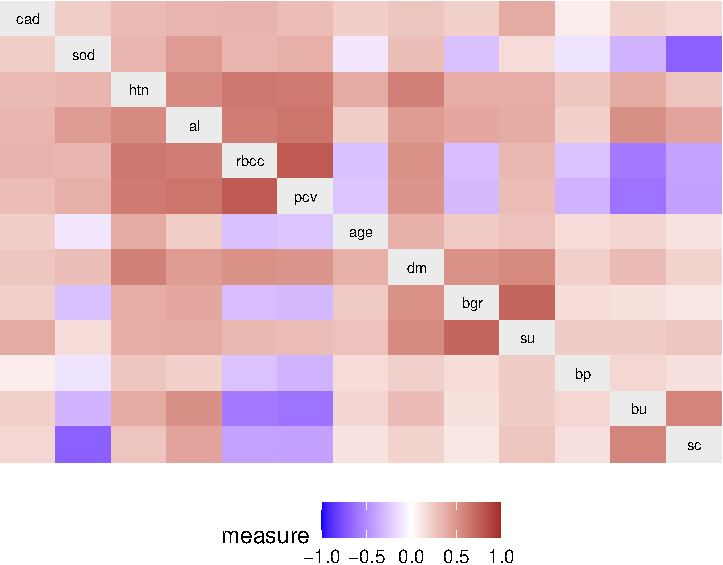
\includegraphics{rj_paper_files/figure-latex/assoc-heatmap-1} 

}

\caption[Association matrix display for penguins data showing Pearson's correlation for numeric variable pairs, canonical correlation for mixed variable pairs and categorical variable pairs]{Association matrix display for penguins data showing Pearson's correlation for numeric variable pairs, canonical correlation for mixed variable pairs and categorical variable pairs.}\label{fig:assoc-heatmap}
\end{figure}
\end{Schunk}

We can also calculate multiple association measures for all the variable
pairs in the dataset and compare them. This will help in finding out
pairs of variables with a high difference among different measures and
one can investigate these bivariate relationships in more detail. The
\texttt{pairwise\_summary\_plot} function can be used to compare various
measures using the matrix layout. It plots multiple measures among the
variable pairs as bars, where each bar represents one measure of
association. Figure \ref{fig:compare-matrix} shows a matrix layout
comparing Pearson's and Spearman's correlation coefficient for the
numeric variable pairs in \emph{penguins} data.

\begin{Schunk}
\begin{figure}

{\centering 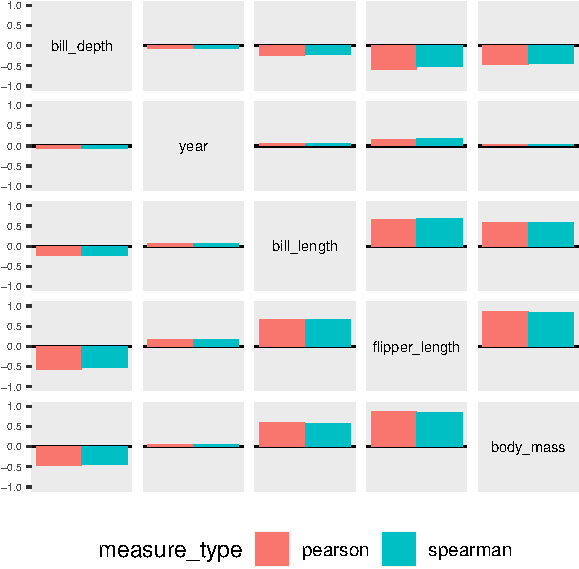
\includegraphics{rj_paper_files/figure-latex/compare-matrix-1} 

}

\caption[Matrix display comparing Pearson's and Spearman's correlation coefficient]{Matrix display comparing Pearson's and Spearman's correlation coefficient. All the variable pairs have similar values for both correlations.}\label{fig:compare-matrix}
\end{figure}
\end{Schunk}

In addition to matrix layout, we can also use linear layouts for
comparing multiple measures. Figure \ref{fig:compare-linear} shows a
linear layout comparing multiple association measures for all the
variable pairs in the penguins data. Linear layouts seems to be more
suitable when comparing high number of association measures.

\begin{Schunk}
\begin{figure}

{\centering 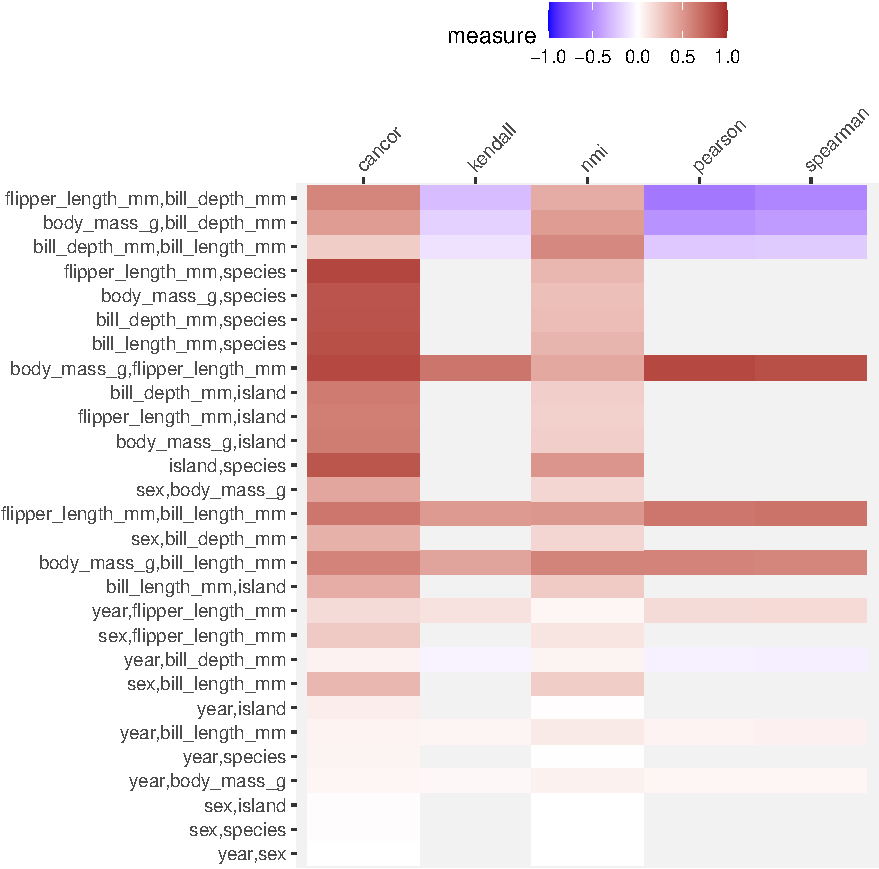
\includegraphics{rj_paper_files/figure-latex/compare-linear-1} 

}

\caption[Comparing multiple association measures using a linear layout]{Comparing multiple association measures using a linear layout. The display has variable pairs on the Y-axis and association measures on the X-axis. The cell corresponding to a variable pair and an association measure has been colored grey showing that the measure is not defined for corresponding pair.}\label{fig:compare-linear}
\end{figure}
\end{Schunk}

\hypertarget{visualising-conditional-association}{%
\subsection{Visualising Conditional
Association}\label{visualising-conditional-association}}

The package includes a function \texttt{calc\_assoc\_by} which
calculates the pairwise association at different levels of a categorical
conditioning variable. This helps in finding out interesting variable
triples which can be explored further prior to modeling. Figure
\ref{fig:cond-assoc} shows a conditional association plot for the
\emph{penguins} data. Each cell corresponding to a variable pair shows
three bars which correspond to the association measure (Pearson's
correlation for numeric pair and Normalized mutual information for other
combination of variables) calculated at the levels of conditioning
variable \emph{island}. The dashed line represents the overall
association measure. The plot shows that there is a high value for
normalised mutual information between bill\_length\_mm and species for
the penguins which lived in \emph{Biscoe} island compared to the
penguins which lived in \emph{Dream} island. It can also be seen that
the cell corresponding to variable pair flipper\_length\_mm and
bill\_depth\_mm has a high negative overall Pearson's correlation and
for the penguins which lived in \emph{Biscoe} island but positive
correlation for penguins which lived in \emph{Dream} and
\emph{Torgersen} island. This is an instance of Simpson's paradox which
can be taken into account during the modeling step.

\begin{Schunk}
\begin{figure}

{\centering 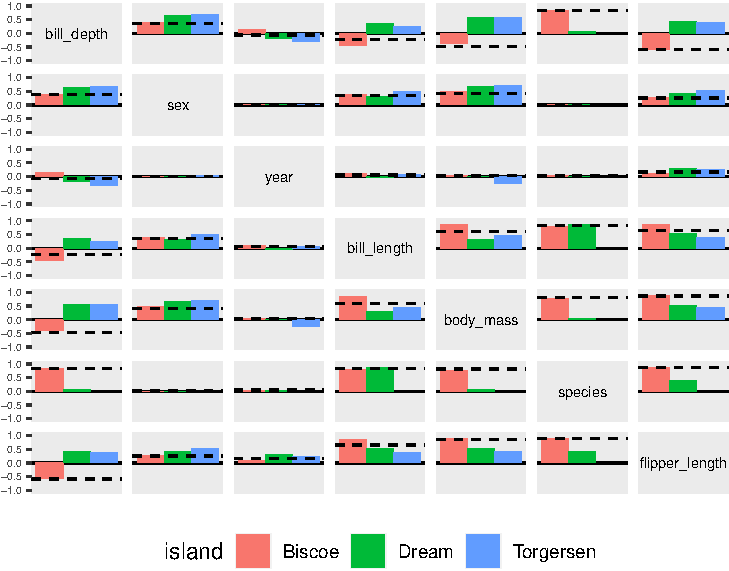
\includegraphics{rj_paper_files/figure-latex/cond-assoc-1} 

}

\caption[Conditional Association plot for penguins data showing Pearson's correlation for numeric pairs and normalised mutual information for categorical or mixed pairs]{Conditional Association plot for penguins data showing Pearson's correlation for numeric pairs and normalised mutual information for categorical or mixed pairs. The bars in each cell represent the value for asssociation measure colored by the conditioning variable `island`. The dashed line in each cell represents overall value of the association measure.}\label{fig:cond-assoc}
\end{figure}
\end{Schunk}

We also provide a functionality for highlighting interesting patterns
like Simpson's paradox. Figure \ref{fig:cond-assoc-sp} shows the matrix
plot with highlighted cells for the variable pairs where Simpson's
paradox is present.

\begin{Schunk}
\begin{figure}

{\centering 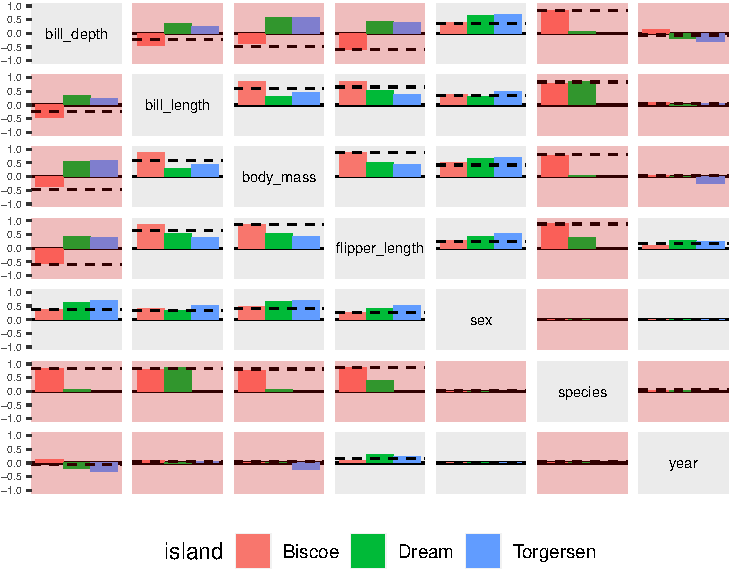
\includegraphics{rj_paper_files/figure-latex/cond-assoc-sp-1} 

}

\caption[Conditional Association plot with examples of Simpson's paradox]{Conditional Association plot with examples of Simpson's paradox}\label{fig:cond-assoc-sp}
\end{figure}
\end{Schunk}

The cells can also be highlighted on the basis of a score calculated by
the user. This can be done by providing a dataframe with pairs of
variables to highlight and a score for highlighting variable pairs. The
cells with high score will have a thicker border compared to cells with
low score. Figure \ref{fig:cond-assoc-manual} shows highlighted cells on
the basis of a score provided for a subset of variable pairs.

\begin{Schunk}
\begin{figure}

{\centering 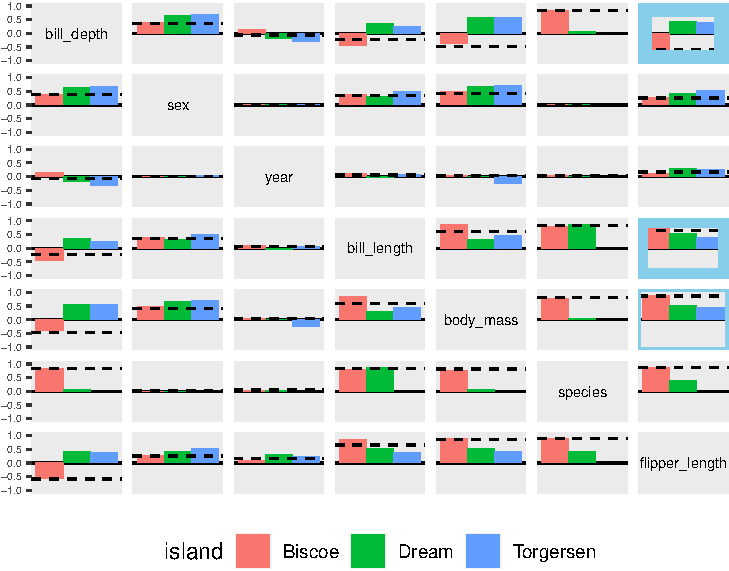
\includegraphics{rj_paper_files/figure-latex/cond-assoc-manual-1} 

}

\caption[Conditional Association plot with manual highlighting]{Conditional Association plot with manual highlighting}\label{fig:cond-assoc-manual}
\end{figure}
\end{Schunk}

We can also use linear layouts for displaying conditional association.
Figure \ref{fig:linear-cond-assoc} shows a funnel-like linear display
for conditional association measures with all the variable pairs on the
y-axis, the value of association measure on x-axis and color of the
points representing the level of the grouping variable. The linear
layout becomes more useful over the matrix layout when the number of
variables and number of levels of grouping variable are high.

\begin{Schunk}
\begin{figure}

{\centering 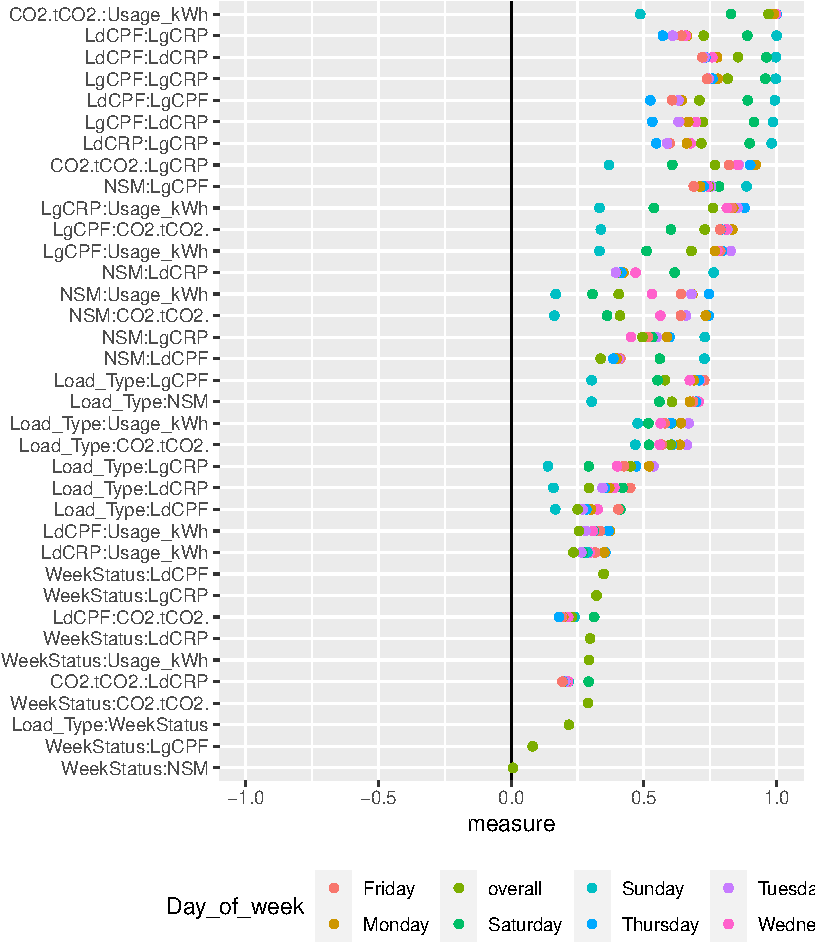
\includegraphics{rj_paper_files/figure-latex/linear-cond-assoc-1} 

}

\caption[Conditional Association plot using linear layout.The display has variable pairs on the Y-axis and the value of association measures on the X-axis]{Conditional Association plot using linear layout.The display has variable pairs on the Y-axis and the value of association measures on the X-axis. The points corresponding to every variable pair represents the value of association measure for different levels of the conditioning variable and the overall value of association measure.}\label{fig:linear-cond-assoc}
\end{figure}
\end{Schunk}

\bibliography{RJreferences.bib}

\address{%
Amit Chinwan\\
Maynooth University\\%
Hamilton Institute\\ Maynooth, Ireland\\
%
%
%
\href{mailto:amit.chinwan.2019@mumail.ie}{\nolinkurl{amit.chinwan.2019@mumail.ie}}%
}

\address{%
Catherine Hurley\\
Maynooth University\\%
Department of Mathematics and Statistics\\ Maynooth, Ireland\\
%
%
%
\href{mailto:catherine.hurley@mu.ie}{\nolinkurl{catherine.hurley@mu.ie}}%
}
